%%%%%%%%%%%%%%%%%%%%%%%%%%%%%%%%%%%%%%%%%%%%%%%%%%%%%%%%%%%%%%%%%%%%%%%%%%%
%%%                                                                     %%%
%%%   LaTeX template voor het verslag van P&O: Computerwetenschappen.   %%%
%%%                                                                     %%%
%%%   Opties:                                                           %%%
%%%     tt1     Tussentijdsverslag 1                                    %%%
%%%     tt2     Tussentijdsverslag 2                                    %%%
%%%     tt3     Tussentijdsverslag 3                                    %%%
%%%     eind    Eindverslag                                             %%%
%%%                                                                     %%%
%%%   2 oktober 2012                                                    %%%
%%%   Versie 1.0                                                        %%%
%%%                                                                     %%%
%%%%%%%%%%%%%%%%%%%%%%%%%%%%%%%%%%%%%%%%%%%%%%%%%%%%%%%%%%%%%%%%%%%%%%%%%%%

\documentclass[tt3]{penoverslag}

%%% PACKAGES
\usepackage{lipsum}
\usepackage{gensymb}
\usepackage [dutch] {babel}
\usepackage{graphicx}
\usepackage{amsmath}
\usepackage{listings}
\usepackage{subcaption}

\begin{document}

% == VOORPAGINA == %
\team{Zilver} % teamkleur
\members{Sam Gielis\\
         Sophie Marien\\
         Toon Nolten\\
         Nele Rober\\
         Gerlinde Van Roey\\
         Maxim Van Mechelen} % teamleden

\maketitlepage

% == ABSTRACT EN INHOUDSTAFEL == %
\begin{abstract}
\label{ssec:abstr} % 3 ok
Het P\&O-project heeft als doel een robot autonoom een doolhof te laten verkennen. Dit verslag beschrijft de invulling die team Zilver aan het project gaf. De robot is voorzien van een lichtsensor en een ultrasone sensor. Deze staan vast gemonteerd en kunnen niet onafhankelijk van de robot bewegen. De aansturing van de robot gebeurt via bluetoothverbinding. Een Grafische User Interface (GUI) maakt deze aansturing op een gebruiksvriendelijke manier mogelijk. De GUI geeft de baan van de robot  weer. Ook de sensorwaarden en een historiek ervan worden weergegeven.\\

De robot kan zich autonoom door een doolhof bewegen zonder op muren te botsen. Tijdens het rijden slaat de robot een map van de doolhof op. Op elke nieuwe tegel kijkt de robot rond zodat muren gedetecteerd kunnen worden door interpretatie van sensorwaarden. Wanneer de hele doolhof verkend is, gebruikt de robot het \textit{A*}-algoritme om de kortste weg naar de finish (via het checkpoint) te bepalen. De finish en het checkpoint worden aangegeven met een bepaalde barcode. Andere barcodes laten de robot een opdracht uitvoeren.\\

Om de afwijking op de aansturing te minimaliseren, ori\"enteert de robot zich regelmatig op een witte lijn. Zo blijft de robot steeds zo dicht mogelijk bij het midden van de tegels.\\

Een computerprogramma simuleert de werking van de robot. Het is voor de simulator mogelijk door een virtuele doolhof te rijden en deze op gelijkaardige wijze te verkennen. De sensorwaarden worden gesimuleerd met een afwijking om de werkelijke robot zo goed mogelijk te benaderen. Verder worden dezelfde algoritmes gebruikt als voor de robot. Dit laat toe de algoritmes te testen zonder de robot hiervoor te gebruiken.
\end{abstract}

%figuur robot
\begin{figure}[!hb]
\begin{flushright}
    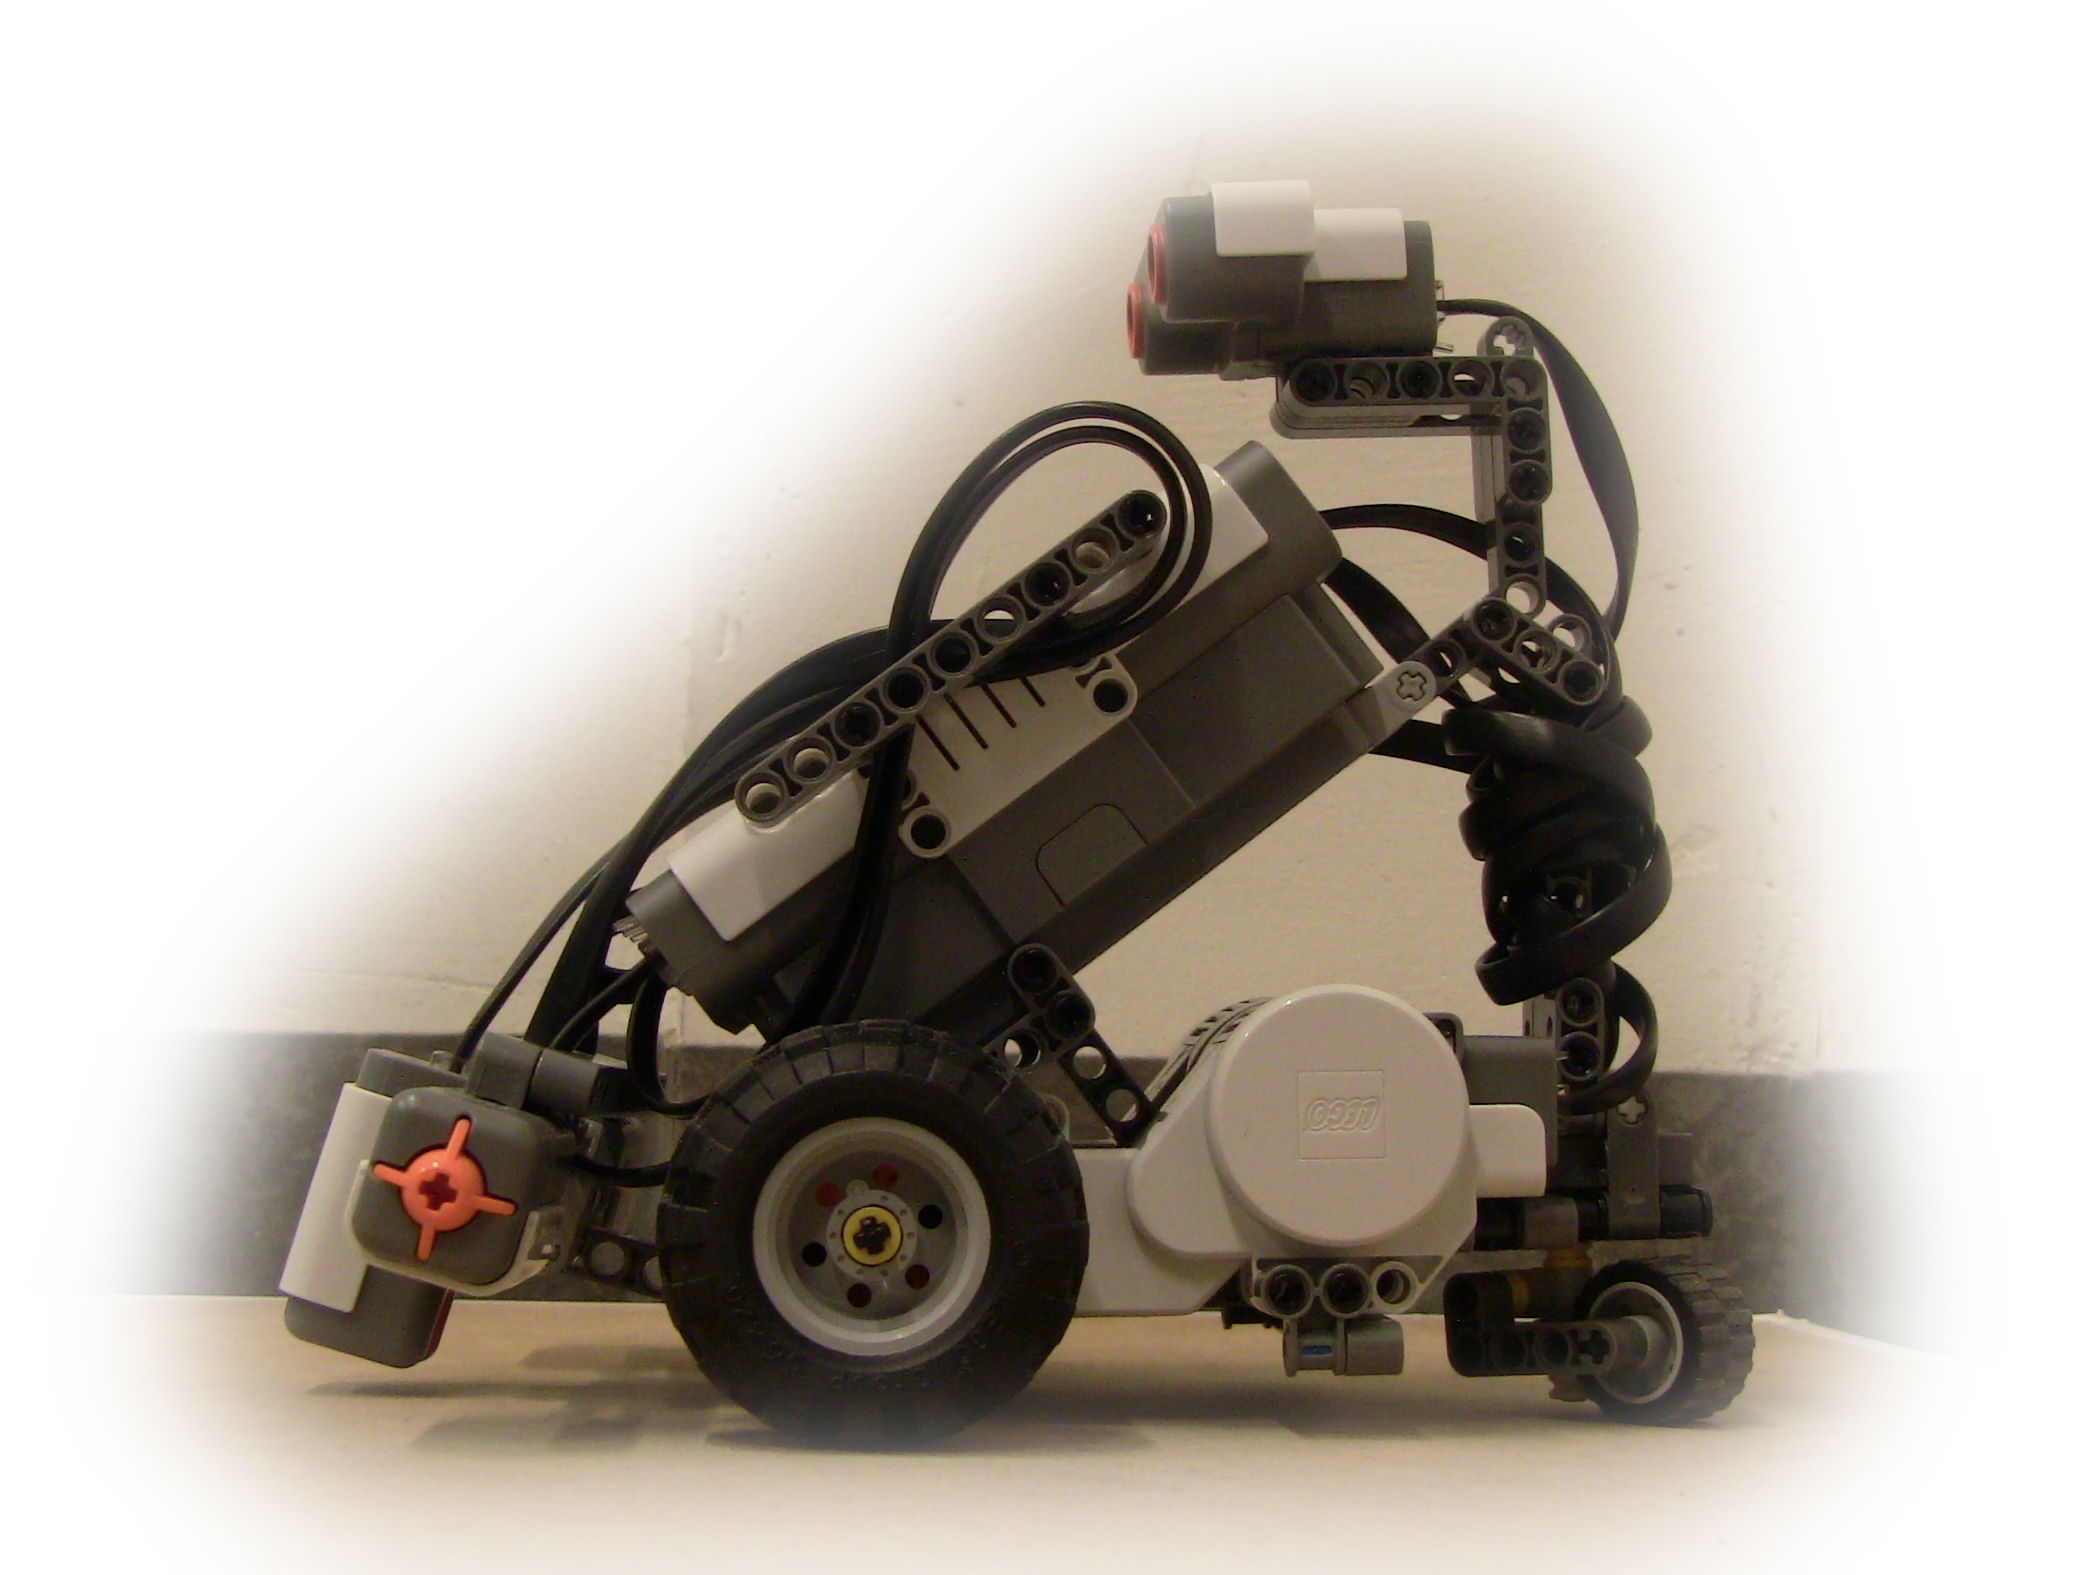
\includegraphics[width=0.8\textwidth]{robotFP}
    \label{fig:robotFP}
\end{flushright}
\end{figure}

\newpage

\tableofcontents
\listoftables
\listoffigures
\thispagestyle{empty}

\newpage 

% == INLEIDING == %
\section{Inleiding} % 3 ok!
\label{ssec:inl}
In het kader van het vak `Probleemoplossen en Ontwerpen: computerwetenschappen' wordt gewerkt rond autonome intelligente robots. Verschillende teams bouwen en programmeren een robot met behulp van LEGO Mindstorms \cite{mindstorms}. Deze robot moet uiteindelijk volledig autonoom een doolhof kunnen verkennen.\\

Op de derde demonstratie kan de robot alle taken van de vorige demonstratie nog steeds uitvoeren. De robot kan zich volledig autonoom voortbewegen. Wanneer de robot zich in een doolhof voortbeweegt, kan hij deze in kaart brengen. Bij het inlezen van barcodes voert de robot een bepaalde opdracht uit. Op het moment dat de volledige doolhof is ingelezen, bepaalt de robot de kortste weg naar de tegel met de barcode `checkpoint'. Vandaar gaat de robot zo snel mogelijk naar de tegel met barcode `finish'.

% == BOUW == %
\section{Bouw van de robot} % 3 ok
\label{sec:bouw}
LEGO Mindstorms \cite{mindstorms} biedt een bouwpakket voor een robot aan. Een NXT-microcomputer laat toe de robot te programmeren. Met behulp van leJOS \cite{leJOS} kan dit in Java.

% == fysieke bouw == %
\subsection{Fysieke bouw} % 3 ok
\label{ssec:fysbouw}
Bij het bouwen van de robot (zie figuur~\ref{robot}) werd het ontwerpboekje gevolgd. Deze compacte samenstelling leek geen directe nadelen te hebben. Twee grote wielen worden elk met hun eigen motor aangestuurd. Een klein wiel achteraan zorgt ervoor dat de robot vlot kan draaien en wordt niet aangedreven. De sensoren (zie figuur~\ref{fig:sensors}) werden als volgt ge\"installeerd: 

\begin{itemize}
\item \textit{lichtsensor:} vooraan en dicht tegen de grond.
\item \textit{ultrasone sensor:} bovenaan, naar voren kijkend; de sensor staat vast gemonteerd.
\item \textit{druksensoren:} aan beide zijkanten, \'e\'en aan de linkerkant en \'e\'en aan de rechterkant.
\end{itemize}

%figuur robot
\begin{figure}[tbp]
\begin{center}
    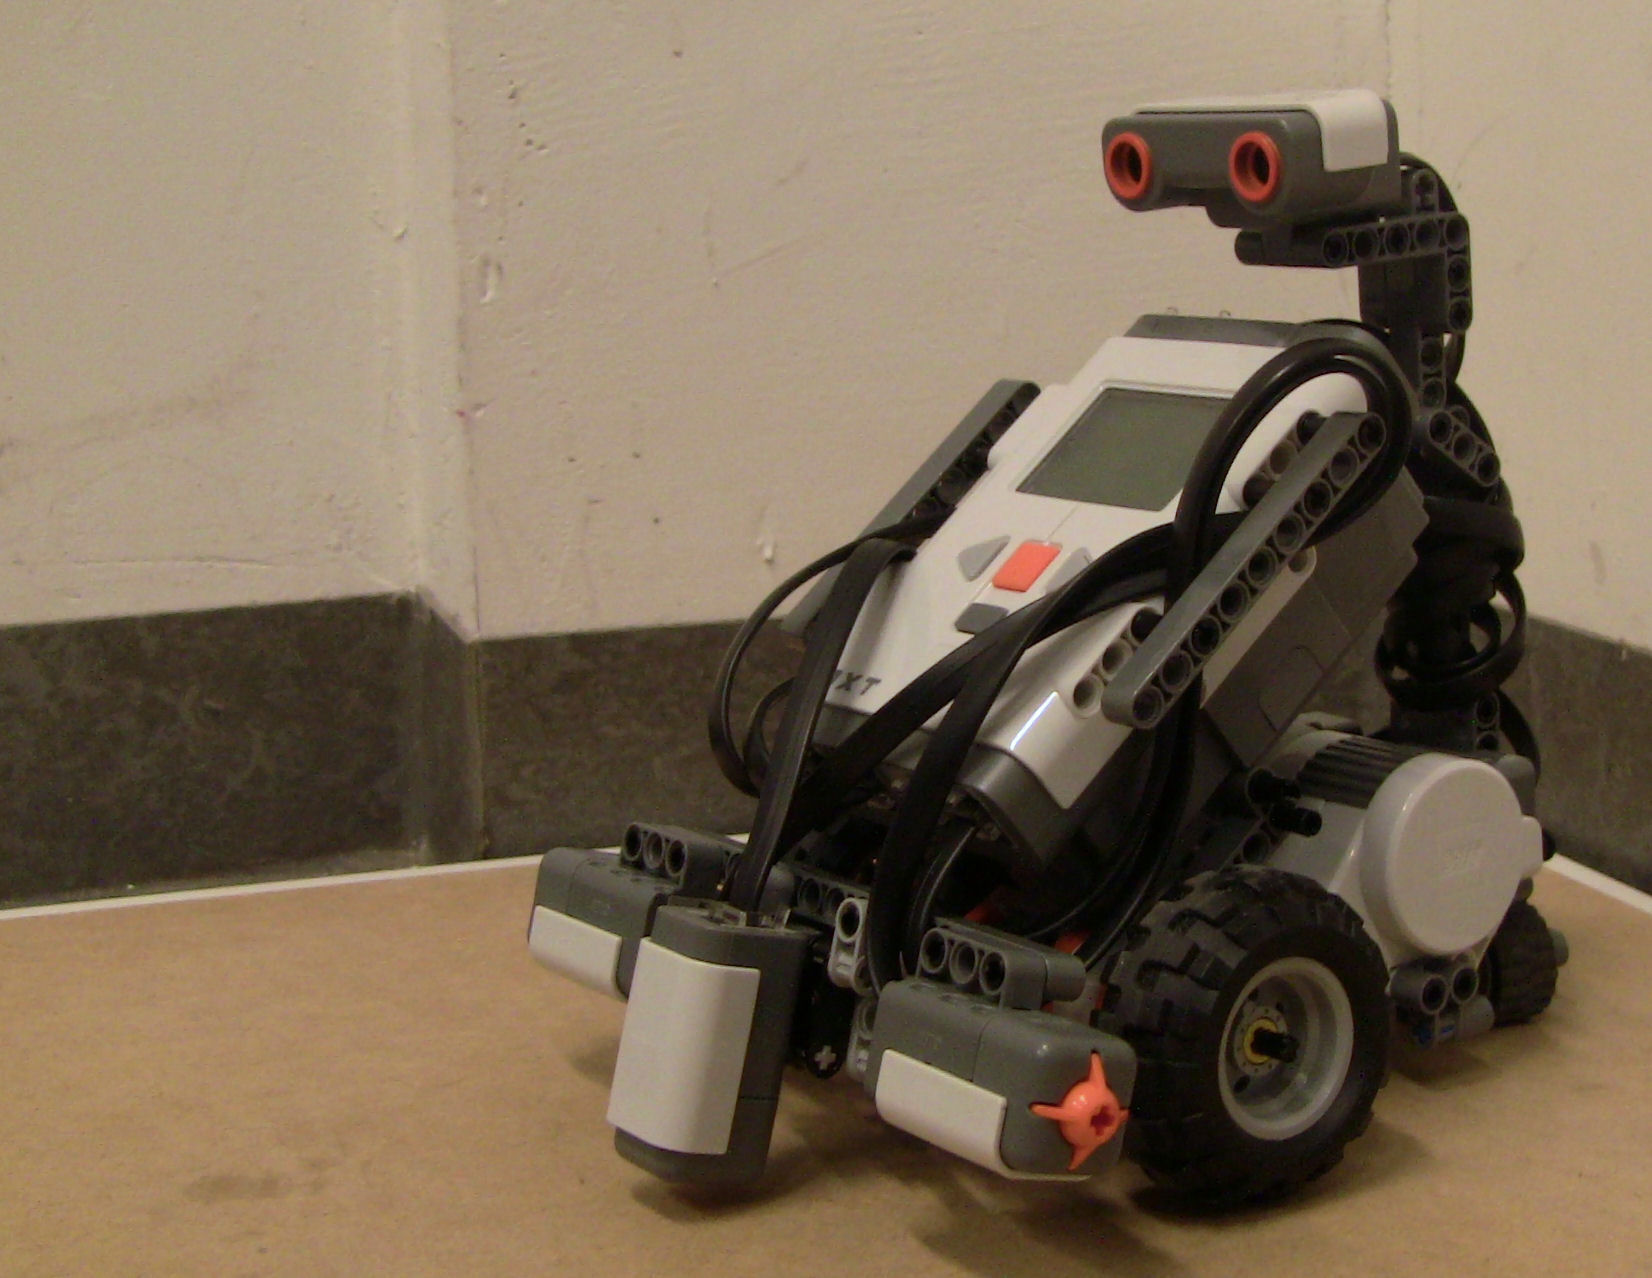
\includegraphics[width=0.5\textwidth]{robot}
    \caption{Robot}
    \label{robot}
\end{center}
\end{figure}

% figuur sensoren
\begin{figure}
        \centering
        \begin{subfigure}[h]{0.54\textwidth}
                \centering
                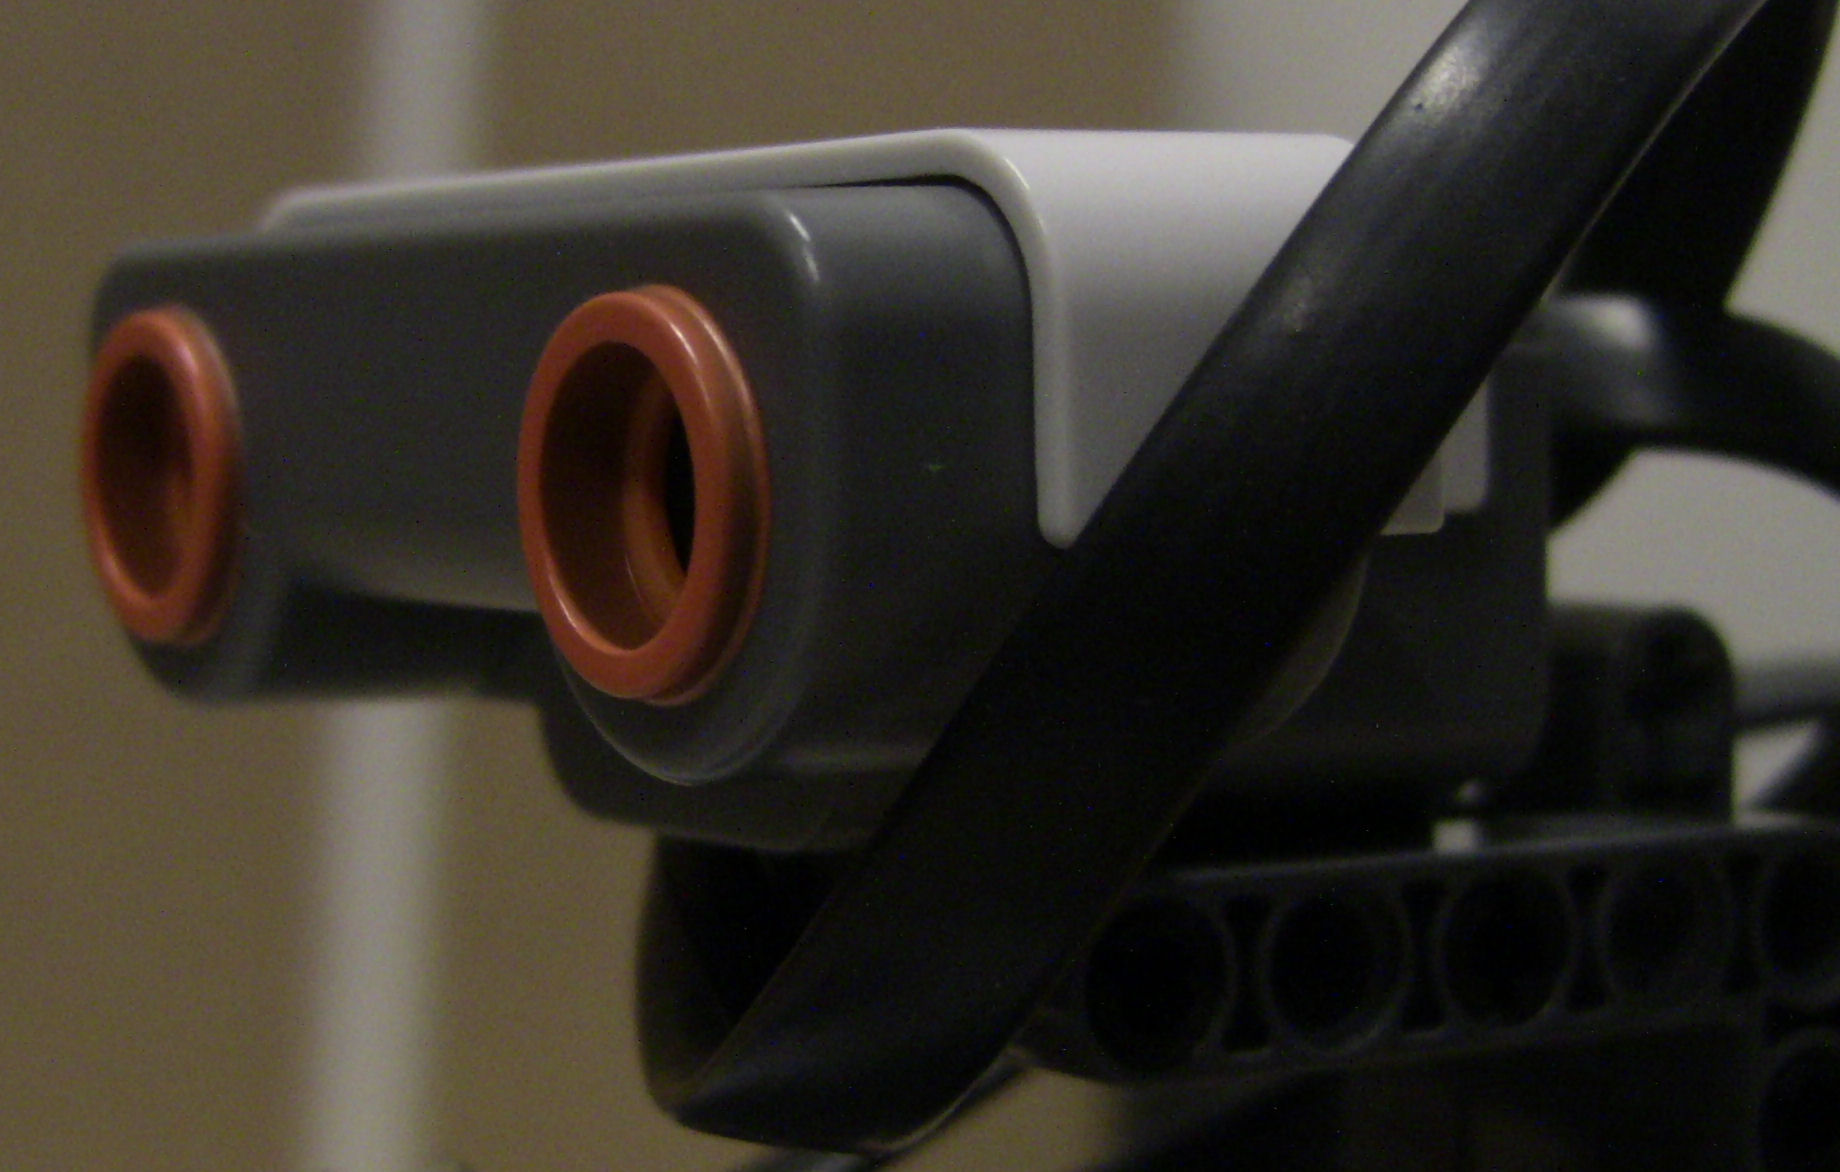
\includegraphics[width=\textwidth]{robotUS}
                \caption{Ultrasone sensor}
        \end{subfigure}%
        \begin{subfigure}[h]{0.46\textwidth}
                \centering
                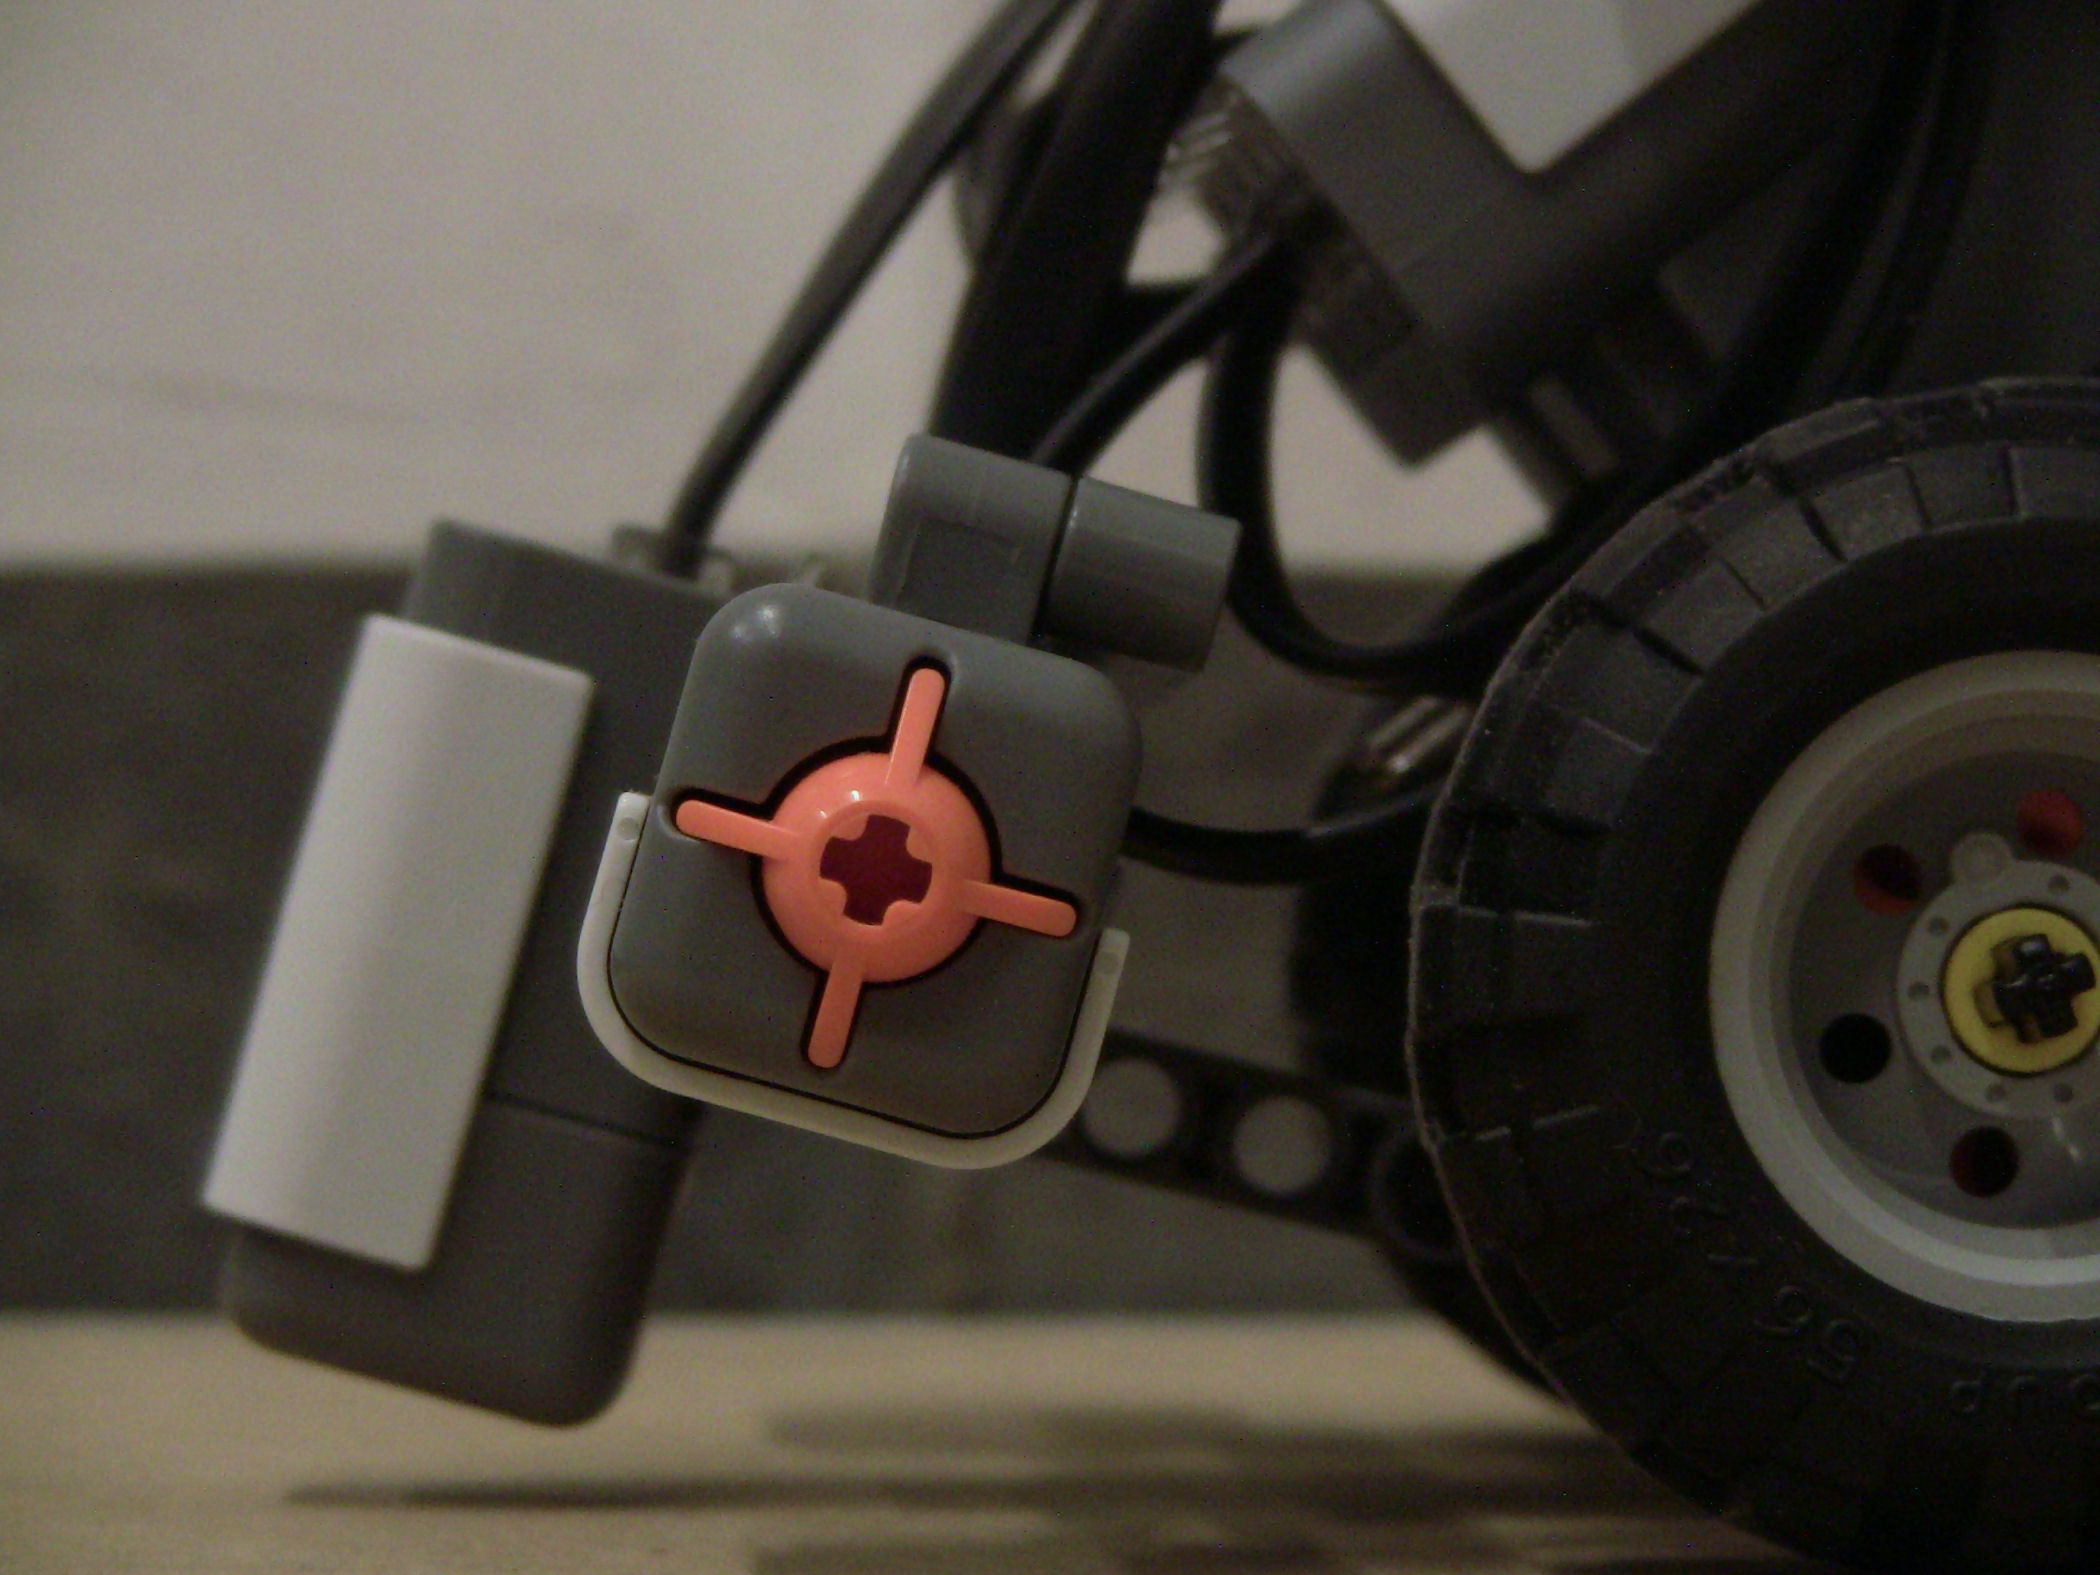
\includegraphics[width=\textwidth]{robotLSTS}
                \caption{Licht- en Druksensor}
        \end{subfigure}
        \caption{Sensoren}
        \label{fig:sensors}
\end{figure}

Een alternatieve opstelling bestaat erin de ultrasone sensor op een derde motor te monteren zodat deze onafhankelijk van de robot kan ronddraaien. De meetwaarde van de ultrasone sensor zou dan afhangen van zijn positie ten opzichte van de robot, wat het interpreteren moeilijker maakt. Voor deze opstelling werd daarom niet gekozen.


% == calibratie == %
\subsection{Calibratie van de motoren} % ok
\label{ssec:calibM}
De robot wordt aangedreven door twee motoren, elk verbonden met \'e\'en van de twee grote wielen. De aansturing gebeurt door te bepalen hoeveel graden de wielen moeten draaien. Beide motoren kunnen onafhankelijk ingesteld worden. De robot kan vooruit bewegen en rond zijn as draaien. De resultaten van de calibratie worden weergegeven in tabel~\ref{tab:resultCalibM}.

%resultaten meetwaarden
\begin{table}[hb]
\begin{center}
    \begin{tabular}{  r || c  c | c }
     & linkerwiel & rechterwiel & aantal graden \\ \hline 
    1 cm vooruit & voor & voor & 20,8\degree
    \\
    1 cm achteruit & achter & achter & 20,8\degree
    \\ \hline
    180\degree draaien linksom & achter & linker & 701\degree \\
    180\degree draaien rechtsom & voor & achter & 701\degree \\
    \end{tabular}
    \caption{Resultaten calibratie motoren}
    \label{tab:resultCalibM}
\end{center}
\end{table}

\subsubsection{E\'en cm vooruit bewegen: bepalen van $x$} % 3 te weinig meetwaarden
\label{ssec:calibMx}
De parameter $x$ bepaalt het aantal graden dat de wielen moeten draaien opdat de robot \'e\'en cm vooruit beweegt.

Een schatting voor $x$ via de $diameter$ (in centimeter) gebeurt als volgt:\\

\begin{equation*}
x_{0} \approx \frac{360}{\pi \cdot diameter}
\end{equation*}\\

Een nauwkeurigere bepaling van $x$ gebeurt via tests.\\
De robot wordt naast een lintmeter geplaatst en krijgt opdracht beide wielen $100 \cdot x$ graden te laten draaien. Bij een perfect gekozen waarde voor $x$, legt de robot precies \'e\'en meter af. Indien niet, wordt $x$ aangepast. De test wordt herhaald tot $x$ een voldoende nauwkeurig resultaat geeft.\\
% ONTBREEKT: x0 + afwijking op 1m; x1 + afwijking; x2 + afwijking + ...

Een volgende test bestaat eruit de robot beide wielen tien maal $10 \cdot x$ graden te laten draaien. Een boxplot van de totaal afgelegde afstand wordt weergegeven in figuur~\ref{fig:calibM}. Wanneer geen afwijking op \'e\'en meter wordt waargenomen, heeft het starten en stoppen van de motoren geen invloed op de totale afgelegde afstand. Dit blijkt echter wel het geval. In verdere algoritmes wordt hier rekening mee gehouden. De robot legt steeds \'e\'en lange afstand af in plaats van vele korte.\\
Uit deze test blijkt bovendien dat de robot een afwijking naar links heeft wanneer hij rechtdoor rijdt. De boxplot van deze afwijking wordt eveneens weergegeven in figuur~\ref{fig:calibM}.
% ONTBREEKT: MEETWAARDEN VAN 1x100CM ter vergelijking


\subsubsection{Volledig rond de as draaien: bepalen van y} % ok
\label{ssec:calibMy}
De parameter $y$ bepaalt het aantal graden dat de wielen moeten draaien opdat de robot 360\degree rond zijn as zou draaien. Beide wielen draaien hierbij in tegengestelde richting.\\
Een schatting voor $y$ via de diameter van het wiel, met $as_{robot}$ (afstand tussen beide wielen) en $diameter$ in centimeter:

\begin{equation*}
y_{0} \approx \frac{(2 \cdot \pi) \cdot (as_{robot}/2)}{diameter_{wiel}/2}
\end{equation*}

De robot wordt naast een lijn geplaatst en krijgt de opdracht zijn wielen $y$ graden in tegengestelde richtingen te laten draaien. $y$ wordt aangepast tot de robot na het draaien opnieuw precies naast de lijn uitkomt.\\
% ONTBREEKT: y0 + afwijking op 360°; y1 + afwijking; y2 + afwijking + ...


Door de robot in stappen rond zijn as te laten draaien ($4 \cdot 90\degree$) kan de invloed van het starten en stoppen van de motoren bepaald worden. Figuur~\ref{fig:calibM} geeft een boxplot van de gemeten afwijkingen op~360\degree. De algoritmes houden rekening met deze afwijking. Wanneer de robot tijdens het verkennen van de doolhof naar \'e\'en kant draait, draait hij, zo mogelijk, evenveel graden naar de andere kant terug. De totale som van de gedraaide graden wordt zo dicht mogelijk bij nul gehouden. Dit maakt de afwijking gedeeltelijk ongedaan. Met de variaties op de afwijking kan echter geen rekening gehouden worden. De algoritmes laten de robot zo weinig mogelijk draaien.
% ONTBREEKT: meetwaarden 1x360° ter vergelijking
% ONTBREEKT: figuur correctie draaien

% boxplots calibratie motoren
\begin{figure}
        \centering
        \begin{subfigure}[h]{0.32\textwidth}
                \centering
                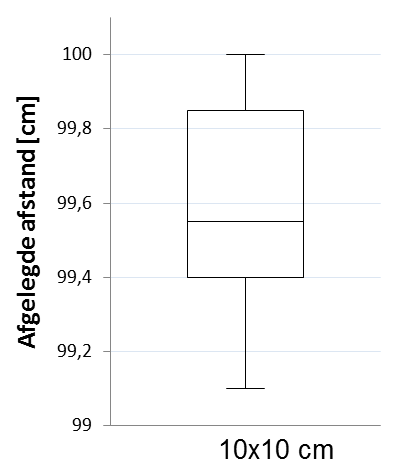
\includegraphics[width=\textwidth]{boxMrechtdoor10x10}
                \caption{Afgelegde afstand rechtdoor}
        \end{subfigure}%
        \begin{subfigure}[h]{0.32\textwidth}
                \centering
                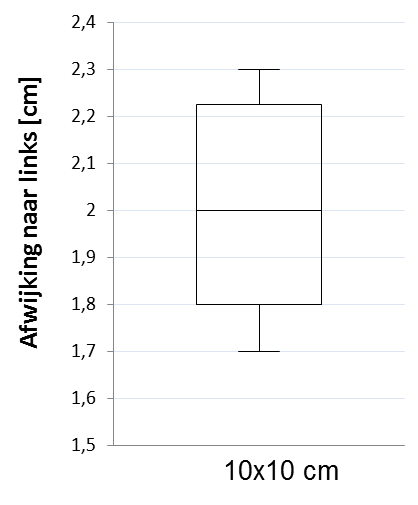
\includegraphics[width=\textwidth]{boxMlinks10x10}
                \caption{Afwijking naar links}
        \end{subfigure}%
        \begin{subfigure}[h]{0.32\textwidth}
                \centering
                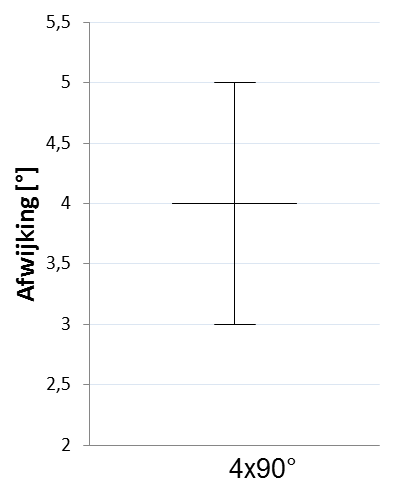
\includegraphics[width=\textwidth]{boxMgraden4x90}
                \caption{Afwijking op $360 \degree$}
        \end{subfigure}
 \caption{Boxplots calibratie motoren}
\label{fig:calibM}
\end{figure}

\subsubsection{Besluit calibratie motoren} %ok
\label{ssec:calibMbesluit}
Uit de tests blijkt dat de robot niet perfect rijdt en draait. Het is daarom nodig regelmatig te corrigeren, zodat de robot toch steeds in het midden van de regels rijdt. Deze correcties worden in de sectie~\ref{ssec:algoWitteL} en~\ref{ssec:algoMuur} beschreven.


\subsection{Calibratie van de lichtsensor} % 3 ok
\label{ssec:calibLS}
De lichtsensor meet de lichtintensiteit van de omgeving. De sensor kan zelf ook een rood licht uitsturen. Hoe minder licht gereflecteerd wordt door de omgeving, hoe donkerder de omgeving. Op deze manier kunnen de meetwaarden ge\"interpreteerd worden als witte of zwarte lijnen.\\
De lichtsensor wordt in verschillende omstandigheden getest: bij direct kunstlicht, in de schaduw, terwijl de robot rijdt en terwijl hij stilstaat. Dit voor alle soorten ondergrond die in de doolhof voorkomen: een paneel, een witte lijn en een zwarte lijn. Boxplots worden weergegeven in figuur~\ref{fig:calibLS}. Deze toont dat het gemiddelde enkel bij een zwarte lijn echt afhangt van de omstandigheden. De afwijking wordt wel sterk bepaald door het al dan niet rijden van de robot. Bij het simuleren en het interpreteren van de meetwaarden wordt hier rekening mee gehouden.

% boxplots calibratie lichtsensoren
\begin{figure}
        \centering
        \begin{subfigure}[h]{0.32\textwidth}
                \centering
                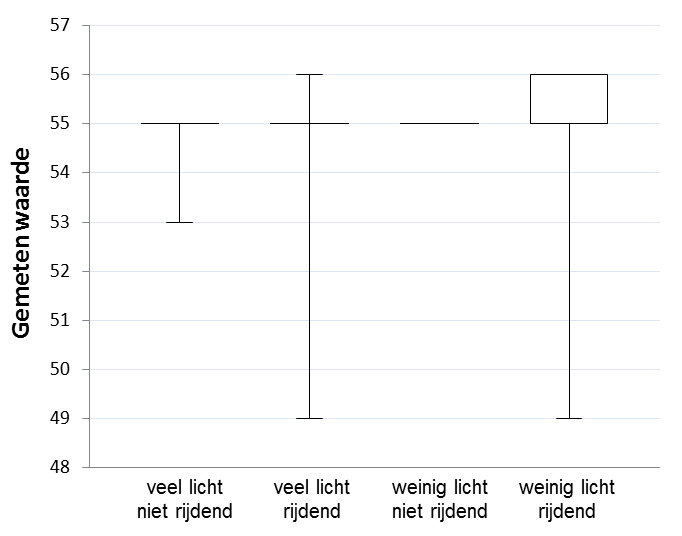
\includegraphics[width=\textwidth]{boxLSwit}
                \caption{Witte lijn}
        \end{subfigure}%
        \begin{subfigure}[h]{0.32\textwidth}
                \centering
                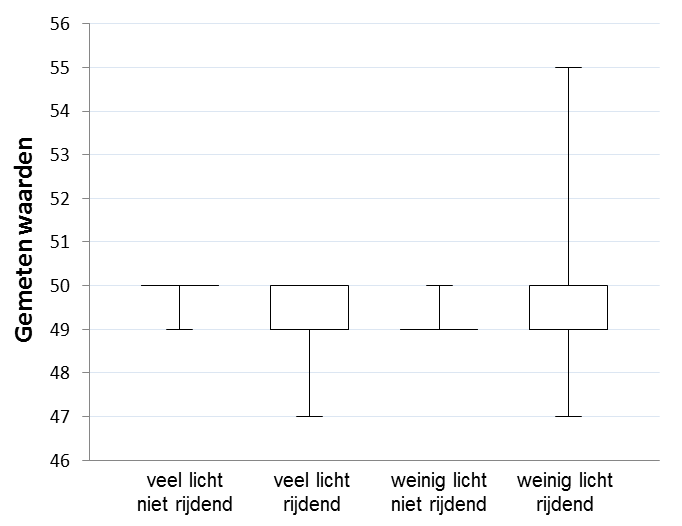
\includegraphics[width=\textwidth]{boxLSpaneel}
                \caption{Paneel}
        \end{subfigure}%
        \begin{subfigure}[h]{0.32\textwidth}
                \centering
                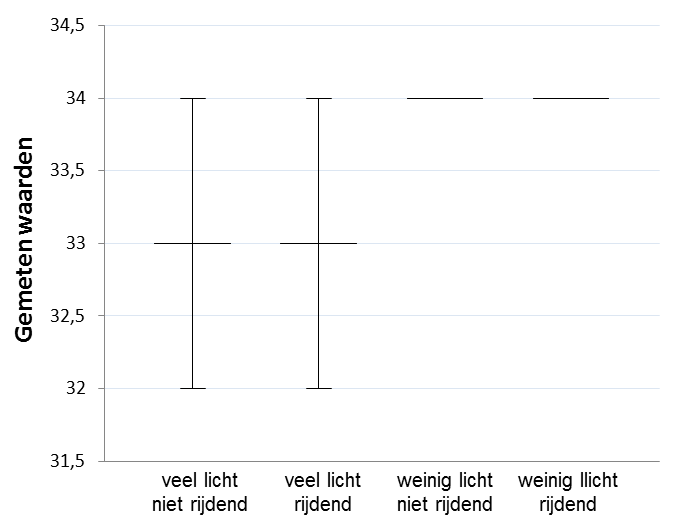
\includegraphics[width=\textwidth]{boxLSzwart}
                \caption{Zwarte lijn}
        \end{subfigure}
 \caption{Boxplots calibratie lichtsensor}
\label{fig:calibLS}
\end{figure}

%%resultaten lichtsensor
%\begin{table}[hb]
%\begin{center}
%    \begin{tabular}{ c | r || c | c | c | c | c | c | c | c }
%     & & WVN & WVR & WWN & WWR & PVN & PVR & PWN & PWR \\ \hline \hline
%    $Q_{0}$ & min & 53 & 49 & 55 & 49 & 49 & 47 & 49 & 47 \\ \hline
%    $Q_{0.25}$ & 1/4 & 55 & 55 & 55 & 55 & 50 & 49 & 49 & 49 \\ \hline
%    $Q_{0.5}$ & med & 55 & 55 & 55 & 55 & 50 & 49 & 49 & 49 \\ \hline
%    $Q_{0.75}$ & 3/4 & 55 & 55 & 55 & 56 & 50 & 50 & 49 & 50\\ \hline
%    $Q_{1}$ & max & 55 & 56 & 55 & 56 & 50 & 50 & 50 & 55 \\ \hline \hline
%     & gem & 54.995 & 55.0261 & 55 & 55.0645 & 49.99688 & 490.2918 & 49.1 & 49.388\\ \hline
%     & st.dev. & 0.10025 & 0.96642 & 0 & 1.025 & 0.055815 & 0.58241 & 0.30015 & 0.95622 \\
%    \end{tabular}
%    \caption{Resultaten lichtsensor, witte ondergrond en paneel ondergrond}
%    \label{tab:resultCalibM}
%\end{center}
%\end{table}
%
%%resultaten lichtsensor
%\begin{table}[hb]
%\begin{center}
%    \begin{tabular}{ c | r ||  c | c | c | c }
%     & & ZVN & ZVR & ZWN & ZWR\\ \hline \hline
%    $Q_{0}$ & min & 32 & 32 & 34 & 34 \\ \hline
%    $Q_{0.25}$ & 1/4 & 33 & 33 & 34 & 34 \\ \hline
%    $Q_{0.5}$ & med & 33 & 33 & 34 & 34 \\ \hline
%    $Q_{0.75}$ & 3/4 & 33 & 33 & 34 & 34\\ \hline
%    $Q_{1}$ & max & 34 & 34 & 34 & 34 \\ \hline \hline
%     & gem & 33.05 & 33.05 & 34 & 34 \\ \hline
%     & st.dev. & 0.27279 & 0.27279 & 0 & 0 \\
%    \end{tabular}
%    \caption{Resultaten lichtsensor, zwarte ondergrond}
%    \label{tab:resultCalibM}
%\end{center}
%\end{table}


\subsection{Calibratie van de ultrasone sensor} % 3 ok
\label{ssec:calibUS}
Een ultrasone sensor zendt ultrasone geluidsgolven uit. Indien een object in de buurt staat, weerkaatsen de golven hierop. De robot ontvangt dan zijn eigen golven. De tijd tussen het uitzenden en ontvangen laat toe de afstand tot het object te bepalen.\\

In een doolhof, kan een robot muren tegenkomen. Ook de paaltjes, die de muren omhoog houden, worden als object gedetecteerd. Om te vermijden dat de paaltjes als muur worden ge"interpreteerd worden enkel meetwaarden kleiner dan 28~cm als muur beschouwd.

Deze 28~cm werd als volgt bepaald: De robot wordt in het midden van een tegel voor een muur geplaatst. De ultrasone sensor meet waarden tussen 12~cm en 24~cm. Vervolgens werd de muur verwijderd en werden er paatjes geplaatst. Nu werden er waarden tussen 32~cm en 50~cm gemeten. Deze metingen leidden tot een grens van 28~cm.\\

De afwijking van de ultrasone sensor wordt gemeten door de robot op een bepaalde afstand van een muur te zetten. Verschillende afstanden worden zo gemeten. Boxplots in figuur~\ref{fig:calibUS} geven de gemeten waarden ten opzichte van de werkelijke waarden weer. Hoewel de variantie op de gemeten waarde niet groot is, komt de gemiddelde gemeten waarde niet altijd overeen met de werkelijke afstand. Vooral voor afstanden kleiner dan 20~cm en groter dan 145~cm. Waarden buiten het interval~[20,145] worden daarom niet als betrouwbaar verondersteld.

% boxplots calibratie ultrasone sensor
\begin{figure}
        \centering
        \begin{subfigure}[h]{0.69\textwidth}
                \centering
                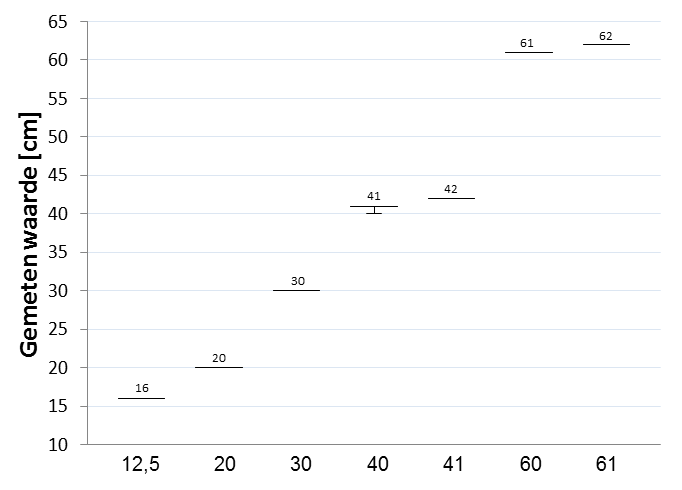
\includegraphics[width=\textwidth]{boxUS}
                \caption[meetwaarden]{meetwaarden (mediaan van de meetwaarden wordt in de figuur weergegeven)}
        \end{subfigure}%
        \begin{subfigure}[h]{0.31\textwidth}
                \centering
                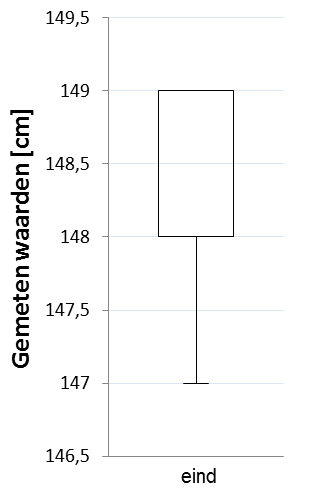
\includegraphics[width=\textwidth]{boxUSeind}
                \caption{laatste geldige meetwaarde}
        \end{subfigure}
 \caption{Boxplots calibratie ultrasone sensor}
\label{fig:calibUS}
\end{figure}

%%resultaten lichtsensor
%\begin{table}[hb]
%\begin{center}
%    \begin{tabular}{ c | r || c | c | c | c | c | c | c | c | c | c | c | c }
%     & & 12.5 & 20 & 30 & 40 & 41 & 60 & 61 & eind\\ \hline \hline
%    $Q_{0}$ & min & 16 & 20 & 30 & 40 & 42 & 61 & 62 & 147 \\ \hline
%    $Q_{0.25}$ & 1/4 & 16 & 20 & 30 & 40 & 42 & 61 & 62 & 148 \\ \hline
%    $Q_{0.5}$ & med & 16 & 20 & 30 & 40 & 42 & 61 & 62 & 149 \\ \hline
%    $Q_{0.75}$ & 3/4 & 16 & 20 & 30 & 40 & 42 & 61 & 62 & 149\\ \hline
%    $Q_{1}$ & max & 16 & 20 & 30 & 40 & 42 & 61 & 62 & 149 \\ \hline \hline
%     & gem & 16 & 20 & 30 & 40.99571 & 42 & 61 & 62 & 148.5 \\ \hline
%     & st.dev. & 0 & 0 & 0 & 0.065512 & 0 & 0 & 0 & 0.565091 \\
%    \end{tabular}
%    \caption{Resultaten ultrasone sensor}
%    \label{tab:resultCalibM}
%\end{center}
%\end{table}


% == ALGORITMES == %
\section{Algoritmes} % 3 ok
\label{sec:algo}
 == veelhoek == %
\subsection{Het rijden van een veelhoek} % 3 ?
\label{ssec:algoVeelH}
De robot en de simulator kunnen beiden een veelhoek rijden. Het aantal hoeken en de lengte van %de zijden kunnen via de GUI ingesteld worden. De robot en de simulator rijden een afstand, %draaien een bepaald aantal graden rond hun as, rijden weer dezelfde afstand,... Tot de %volledige veelhoek gereden is. 

\lstset{frame=single, language=Java, caption=Veelhoek algoritme (pseudocode),
   	label=code:algoVeelH, numbers=left, numberstyle=\footnotesize,
		basicstyle=\sffamily, numbersep=5pt}
\begin{lstlisting}
Angle = (360.0/amtOfAngles)*100
Voor i van 0 tot amtOfAngles
	Beweeg lengthInCM vooruit
	Draai angle
\end{lstlisting}


% == witte lijn == %
\subsection{Rechtzetten op een witte lijn} % 3 ok
\label{ssec:algoWitteL}
Indien regelmatig gecorrigeerd wordt op de calibratieafwijkingen kan de impact ervan geminimaliseerd worden. Deze correctie gebeurt onder andere door de witte lijnen als referentie te nemen en hier loodrecht op te ori\"enteren. List De robot rijdt dan weer rechtdoor. Listing~\ref{code:algoWitteL} toont een algoritme dat gebruikt kan worden wanneer de robot net over een witte lijn staat (wanneer hij volledig rond zijn as draait zou hij de witte lijn moeten detecteren).

\lstset{frame=single, caption=Witte Lijnalgoritme (pseudocode),
		label=code:algoWitteL, numbers=left, numberstyle=\footnotesize,
		basicstyle=\sffamily, numbersep=5pt}
\begin{lstlisting}
AngleTurned = 0

Draai(rechts,5) tot witte lijn.
Draai(links,1) tot witte lijn EN AngleTurned++.
Draai(rechts, AngleTurned/2).
\end{lstlisting}
%ONTBREEKT: figuur

De robot staat best net over de witte lijn. Wanneer de robot dan op een witte lijn tussen twee panelen staat, zorgt de donkere scheidingslijn tussen twee panelen niet voor verwarring.\\

Dit algoritme wordt tijdens het verkennen en tijdens het rijden naar de finish uitgevoerd. De robot zet zich elke vijf tegels recht.
% ONTBREEKT: elke vijf? of vaker?

% == muren == %
\subsection{Centreren aan de hand van twee muren} % 3 ok
\label{ssec:algoMuren}
Een alternatieve manier om te corrigeren op calibratieafwijkingen is door gebruik te maken van muren. Met dit algoritme zet de robot zich in het midden van een tegel. De robot kijkt naar een muur en meet op hoeveel afstand hij zich van de muur bevindt. Hij rijdt eventueel wat naar voren en meet dan de afstand tot de tegenovergestelde muur. Eventueel rijdt hij weer wat naar voren. Het algoritme is enkel toepasbaar wanneer de robot zich op een tegel met muren aan twee kanten bevindt.

\lstset{frame=single, caption=Muuralgoritme (pseudocode),
		label=code:algoWitteL, numbers=left, numberstyle=\footnotesize,
		basicstyle=\sffamily, numbersep=5pt}
\begin{lstlisting}
Draai(rechts,90)
ALS     ultraSensor() < 28
DAN 	Rijd(ultraSensor()-23)
    	Draai(links,180)
    	ALS 	ultraSensor() < 28 EN ultraSensor() NIET in [21,25]
        DAN 	Rijd(ultraSensor()-23)
		Draai(rechts,90)
		
ANDERS 	Draai(links,180)
	ALS 	ultraSensor() < 28
	DAN     Rijd(ultraSensor()-23)
       	        Draai(rechs,90)
	ANDERS	Draai(rechts,90)
\end{lstlisting}
%ONTBREEKT: figuur

Dit algoritme wordt uitgevoerd op tegels met barcodes. Zo zijn er zeker muren aan weerskanten. Het algoritme wordt niet uitgevoerd tijdens het rijden naar de finish.

% == barcodes lezen == %
\subsection{Lezen van een barcode} % 3 ok
\label{ssec:algoBarcode}
Een \textit{Barcode} bestaat uit acht stroken van twee~cm breed. De eerste en de laatste strook zijn altijd zwart. De tussenin liggende stroken zijn ofwel zwart (waarde nul) ofwel wit (waarde \'e\'en). Deze combinatie van enen en nullen is een binaire voorstelling van een integer.

De klasse \textit{BarDecoder} zet de integer om in de juiste opdracht. Ook indien de \textit{Barcode} in de andere richting gelezen werd, wordt de juiste opdracht toegekend.\\

Zowel de robot als de simulator hebben een \textit{BarcodeThread} die checkt of er een zwarte ondergrond is. Dit gebeurt terwijl de robot rijdt. Bij detectie van een zwarte ondergrond, wordt het barcodealgoritme opgeroepen.

Aan de start van het barcodealgoritme staat de robot op de eerste zwarte strook. De robot rijdt twee~cm vooruit, leest de waarde van zijn lichtsensor en interpreteert de waarde van de strook. Zo tot alle stroken gedetecteerd zijn. De waarde van de barcode wordt opgeslagen in de map van de doolhof. Nadien rijdt de robot nog vier~cm vooruit zodat hij de barcode zeker voorbij is. Het muuralgoritme wordt opgeroepen en daarna wordt de opdracht bij de barcode uitgevoerd.


% == verkennen van de doolhof == %
\subsection{Verkennen van een doolhof} % 3 ok
\label{ssec:algoOnderzDoolhof}

De robot kan een volledige doolhof autonoom verkennen. Elke tegel die de robot passeert, wordt gemarkeerd. Indien alle tegels gemarkeerd zijn, is de volledige doolhof doorzocht. Elke tegel houdt een boolean bij die deze markering voorstelt.

Bij elke tegel onthoudt de robot alle uitwegen (de naburige tegels). Vervolgens slaat hij de laatste nog-niet-bekeken uitweg in. Wanneer de robot op een doodlopend stuk komt, keert hij terug tot een kruispunt waar nog niet alle uitwegen van bekeken werden. De robot gebruikt het kortste pad algoritme om de weg naar dit kruispunt te bepalen.
Nadat de robot het hele doolhof bekeken heeft, kijkt hij na of de doolhof een `finish'-barcode en een `checkpoint'-barcode bevat. Indien niet, dan stopt de robot en voert hij het kortste pad algoritme niet uit.\\

Enkele optimalisaties werden doorgevoerd in het algoritme. De genoemde aanpassing implementeert steeds ook de aanpassingen die eerder werden toegevoegd. Tabel~\ref{tab:resultVerken} geeft de resultaten van de aanpassingen weer. Figuur~\ref{fig:resultVerkenE} toont de gebruikte doolhoven en de uitvoering van het algoritme met aanpassing E. Er werd getracht het aantal draaiingen en afgelegde afstand te minimaliseren.
\begin{description}
\item[A] basisalgoritme zonder optimalisatie: draai bij elke tegel vier keer (eindig in startori\"entatie) en neem de laatste tile in de queue als volgende tile.
\item[B] neem steeds de buur die met het minst aantal rotaties bereikt kan worden als volgende tile.
\item[C] draai bij elke tegel slechts drie keer (eindig niet meer in startori"entatie).
\item[D] muren die vanuit een naburige tile reeds gedetecteerd werden, worden niet nog eens nagekeken.
\item[E] tiles waarvan de vier zijden al gekend zijn en waaraan drie muren grenzen, worden niet meer bezocht (`dead-ends' kunnen onmogelijk barcodes bevatten, dus dit is geen probleem)
\end{description}

%resultaten lichtsensor
\begin{table}[!hb]
\begin{center}
    \begin{tabular}{ c ||  c | c | c | c }
     & \multicolumn{2}{|c|}{map 1}& \multicolumn{2}{|c}{map 2} \\
    optimalisatie & \degree gedraaid & cm afgelegd & \degree gedraaid & cm afgelegd\\ \hline \hline
    A & 14400 & 2160 & 10620 & 1080 \\ \hline
    B & 13770 & 1920 & 10800 & 1160 \\ \hline
    C & 11970 & 2000 & 9090 & 1080 \\ \hline
    D & 9180 & 2000 & 6570 & 1080\\ \hline
    E & 8820 & 1880 & 6570 & 1080\\
    \end{tabular}
    \caption{Testen algoritmes}
    \label{tab:resultVerken}
\end{center}
\end{table}

% figuren verkenning doolhof
\begin{figure}
        \centering
        \begin{subfigure}[hb]{0.64\textwidth}
                \centering
                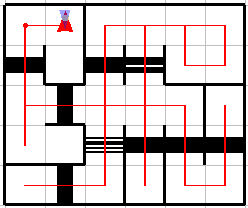
\includegraphics[width=\textwidth]{verkenMap1E}
                \caption{map 1}
        \end{subfigure}%
        \begin{subfigure}[hb]{0.36\textwidth}
                \centering
                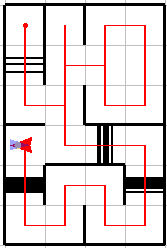
\includegraphics[width=\textwidth]{verkenMap2E}
                \caption{map 2}
        \end{subfigure}
 \caption[Verkennen van een doolhof]{Verkennen van een doolhof met implementatie van aanpassing E. Deze aanpassing maakt dat in map 1 niet alle tegels bezocht hoeven te worden. In map 2 doet deze situatie zich niet voor. Dit is te wijten aan de opbouw van de doolhof.}
\label{fig:resultVerkenE}
\end{figure}

% == het kortste pad == %
\subsection{Vinden van het kortste pad} % ?
\label{ssec:AlgoKortsteP}

%figuur kortste pad
\begin{figure}[tbp]
\begin{center}
    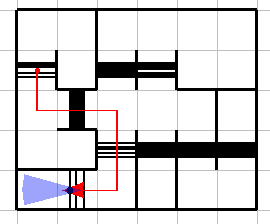
\includegraphics[width=0.8\textwidth]{kortstepadvisual}
    \caption{Kortste padalgoritme}
	\label{fig:kortstepad}
\end{center}
\end{figure}

Het kortste padalgoritme implementeert \textit{A*} \cite{A*}. Het maakt gebruik van een graaf die opgesteld wordt tijdens het verkennen van het doolhof. Als heuristiek wordt de Manhattanafstand \cite{manhattan} ge\"implementeerd (zonder rekening te houden met muren) en als kost de totale afgelegde afstand (wel rekening houdend met muren). Figuur \ref{fig:kortstepad} toont een uitvoering van het algoritme.

Dit algoritme markeert alle tegels die al onderzocht zijn (dit is een andere mark dan het verkenalgoritme). In de beginsituatie zijn alle tegels ongemarkeerd. De kost van de startpunt wordt op nul gezet. Daarna wordt de kost opbouwend aan elke tegel meegegeven.

% == SOFTWARE == %
\section{Software} % 3 ok
\label{sec:softw}
De software bestaat uit twee delen: een project dat op de NXT van de robot loopt (sectie \ref{ssec:robot}) en een project dat op de computer loopt (sectie \ref{ssec:Sdesign}). Alles wordt aangestuurd via de \textit{Graphical User Interface (GUI)} (sectie \ref{ssec:GUI}) . Deze toepassing laat toe de robot te besturen (via bluetooth: sectie \ref{ssec:bluetooth}) en de reacties van de robot weer te geven. Via de GUI kan ook een virtuele robot aangestuurd worden: de simulator (sectie \ref{ssec:simulator}). Een \textit{Communication}-pakket stuurt de commando's van de GUI door naar de juiste unit (sectie \ref{ssec:commands}). Wanneer robot of simulator een doolhof verkennen wordt een map opgebouwd met behulp van het \textit{Mapping}-pakket (sectie \ref{ssec:mapping}).\\

% == software design == %
\subsection{Ontwerp van het computerproject} % 3 ?
\label{ssec:Sdesign}
Zoals reeds vermeld bestaat de software uit twee projecten: \'e\'en draait op een computer en \'e\'en draait op de NXT-Brick. Figuur~\ref{fig:klasDia} toont een vereenvoudigd klassendiagram van de software op de computer. De gebruiker geeft zijn commando's door aan de \textit{GUI}. Deze stuurt de commando's weer door naar de \textit{Communicator} die verder doorstuurt naar ofwel de robot ofwel de simulator. De \textit{Simulator} en de \textit{Robot} geven hun sensorwaarden door aan de \textit{Informationbuffer}. De \textit{Informatiebuffer} stuurt ze weer door naar de \textit{GUI} zodat deze de sensorwaarden kan weergeven.\\
%
%Beide projecten hebben een identiek package \textit{Commands} met \'e\'en klasse \textit{Command}. Hierin staan de final static integers die met de mogelijke bluetoothsignalen overeenkomen. Een verdere beschrijving van de software op de NXT-brick wordt in de sectie robot gegeven.\\
%
%
%Het computerproject heeft nog zes andere packages: \textit{communication}, \textit{gui}, \textit{simulator}, \textit{mazeAlgorithm}, \textit{audio} en \textit{mapping}. 
%De klasse \textit{SilverSurferGUI} uit de package \textit{gui} implementeert de GUI. De GUI communiceert met de simulator of de robot via de klassen in het package \textit{communication} door een object van de superklasse \textit{UnitCommunicator} bij te houden.\\
%
%Andere klassen van de package \textit{gui} zijn: \textit{MouseClickThread} , \textit{PolygonDrawThread}, \textit{RunForwardThread} en \textit{TurnAngleThread}. De vier Threads zorgen ervoor dat het tekenen van de baan van de robot de rest van het programma niet stillegt. \\

%figuur klassendiagram PC
\begin{figure}[tbp]
\begin{center}
    \includegraphics[width=0.8\textwidth]{Klassendiagram}
    \caption{Klassendiagram van het computerproject.}
    \label{fig:klasDia}
\end{center}
\end{figure}

% == gui == %
\subsection{Grafische User Interface} % 3 ok
\label{ssec:GUI}
De GUI toont een grafische weergave van de doolhof en de baan die de robot erin aflegt: zie figuur~\ref{fig:gui}. De sensorwaarden worden grafisch weergegeven: een bolletje op de robot geeft de kleur van de ondergrond aan en een blauwe straal toont het bereik van de ultrasone sensor. Grafieken tonen de historiek van de ultrasone sensor en de lichtsensor. Figuur~\ref{fig:guiSensoren} toont zowel de grafische weergave als de grafiek. \\

Via de GUI kan de gebruiker de robot of de simulator aansturen, naargelang de bluetooth geactiveerd is. Het is mogelijk virtuele doolhoven te laden en te verkennen. Gemeten sensorwaarden kunnen ge\"exporteerd worden naar een text-file. Bovendien is het mogelijk in de zoomen op de robot en kan met het scherm geschoven worden.

%figuur gui
\begin{figure}[tbp]
\begin{center}
    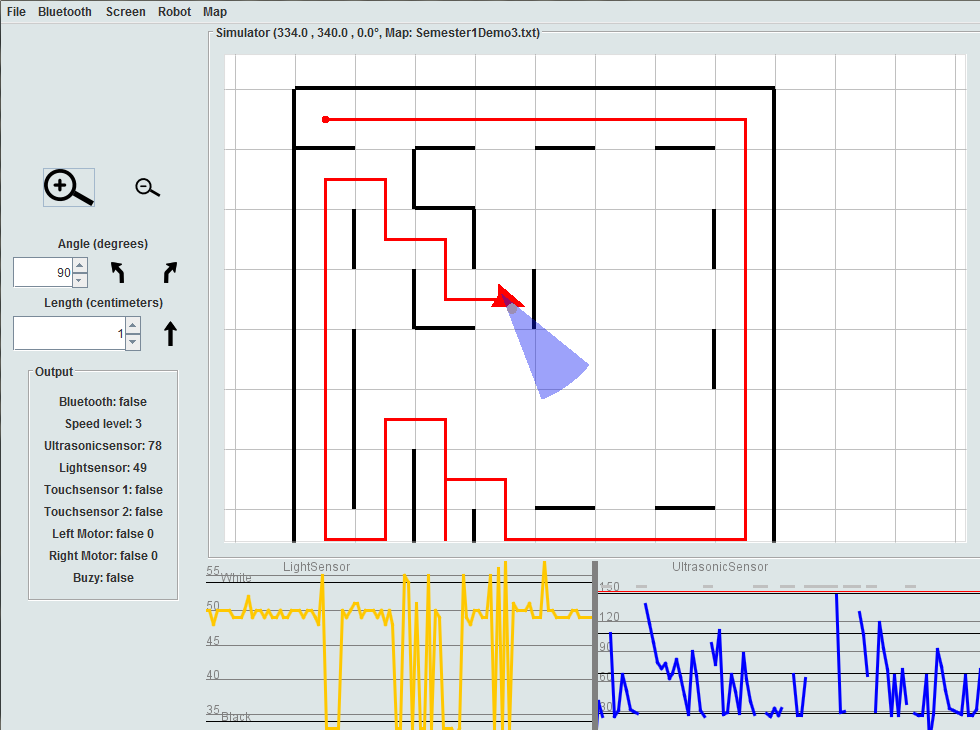
\includegraphics[width=0.8\textwidth]{GUI}
    \caption{Grafische User Interface}
	\label{fig:gui}
\end{center}
\end{figure}

% figuren weergave sensoren
\begin{figure}
        \centering
        \begin{subfigure}[hb]{0.25\textwidth}
                \centering
                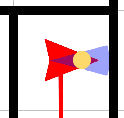
\includegraphics[width=\textwidth]{guiRobot}
                \caption{grafisch}
        \end{subfigure}%
        \begin{subfigure}[hb]{0.75\textwidth}
                \centering
                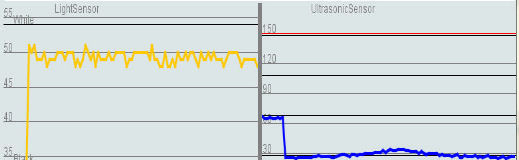
\includegraphics[width=\textwidth]{guiSensor}
                \caption{grafieken}
        \end{subfigure}
 \caption{Weergave van de sensorwaarden}
\label{fig:guiSensoren}
\end{figure}

% == commando's == %
\subsection{Het doorgeven van commando's} % 3 ok!
\label{ssec:commands}
De GUI zet een actie van de gebruiker om in een commando. Dit commando wordt vertaalt naar een integer die naar de klasse \textit{UnitCommunicator} wordt gestuurd. Twee van de commando's hebben echter extra informatie nodig: \textit{automatic move $x$ cm forward} en \textit{rotate $x$ degrees}. Deze informatie wordt toegevoegd aan de integer door de integer uit te breiden met extra cijfers.\\

\subsubsection{Bewerking op de integers} % 3 ok!
\label{sssec:integer}
Integers stellen de commando's voor. In twee gevallen is echter meer informatie nodig: om de robot een bepaalde afstand te laten afleggen en om de robot een bepaald aantal graden te laten draaien. Deze afstand en dit aantal graden moet mee doorgegeven worden met de integer. De eenheden waarin de afstand en de hoek worden doorgestuurd zijn respectievelijk cm en graden.

De doorgegeven integer wordt als volgt opgebouwd:

\begin{itemize}
\item de waarde van de afstand (hoek) wordt vermenigvuldigd met 1000.
\item de integer die het commando representeert, wordt hierbij opgeteld.
\end{itemize}

Om de bekomen resultaten terug op te splitsen in de twee oorspronkelijke gegevens worden volgende stappen gevolgd:

\begin{itemize}
\item een modulo-operatie van honderd geeft het laatste cijfer terug. Dit stelt het soort commando voor.
\item dit getal wordt van de integer terug afgetrokken.
\item de oorspronkelijke afstand (hoek) wordt bekomen door de integer door 1000 te delen.
\end{itemize}

Deze werkwijze brengt een beperking met zich mee: de waarde van de afstand (hoek) kan slechts tot twee cijfer(s) na de komma doorgegeven worden. De robot kan niet nauwkeuriger dan 0,1~cm aangestuurd worden. Hierdoor is het niet nodig de afstand nauwkeuriger door te geven. De nauwkeurigheid van de hoek is gevoeliger. De veelhoek stapelt immers veel afrondingsfouten op naarmate de lengte van de zijde en/of het aantal hoeken stijgt. Doordat de begin- en eindpunten niet samenvallen is te zien dat de som van de berekende hoeken samen geen 360~graden vormt. 

% == bluetooth == %
\subsection{Bluetooth} % 3 ok!
\label{ssec:bluetooth}
De communicatie tussen robot en computer gebeurt volledig via bluetooth. De GUI voorziet een knop om deze verbinding te maken en geeft de status van de verbinding weer. De GUI stuurt commando's door naar de robot via de \textit{Communicator}-klassen.\\

De leJOS-API \cite{leJOS} voorziet een \textit{NXTConnector} klasse. De methode \textit{connectTo((String, String, int, int)} zet de bluetoothverbinding tussen computer en brick op. De belangrijkste argumenten hiervoor zijn de naam van de NXT-Brick en zijn DeviceUrl  - in het geval van de gebruikte NXT: `Silver' en `00:16:53:0A:04:5A'.\\

De bluetooth laat toe twee `datastreams' tussen robot en computer op te zetten: een inputstream en een outputstream. Alle informatie wordt hierover doorgestuurd in de byte-voorstelling van een string. Op de Die bytes worden bij aankomst weer omgezet naar een string. De computer interpreteert die aan de hand van tags die vooraan de string staan. Naast de tags worden enkel integers doorgestuurd.

% == robot == %
\subsection{Robot} % 3 ok
\label{ssec:robot}
Het project op de NXT-brick bestaat uit een klasse \textit{CommandUnit}, een klasse \textit{Command} en enkele threadklassen. Deze laatsten maken het mogelijk meerdere dingen tegelijk te doen (bijvoorbeeld: sensorwaarden inlezen terwijl de robot rijdt). Bij het opstarten, initialiseert de robot zijn sensoren. Wanneer de computer verbinding maakt, initialiseert de robot ook zijn `datastreams' en start hij een \textit{SensorThread} op.

De computer stuurt commando's in de vorm van integers. De robot vertaalt deze met behulp van de klasse \textit{Command} en voert de juiste actie uit. Sommige methodes retourneren een waarde aan de computer. Dit gebeurt door de waarde op een `datastream' te zetten, voorafgegaan door een tag (bijvoorbeeld: [US] voor ultrasonesensor data).\\

Enkele belangrijke methodes van \textit{CommandUnit}:
\begin{itemize}
\item \textit{updateCoordinates:} de robot houdt zijn positie bij. Bij elke beweging zullen de co\"ordinaten worden ge"updatet.
\item \textit{updateStatus:} stuur alle statusgegevens (lichtsensor, co\"ordinaten, ...) naar de computer.
\item \textit{main:} wacht tot de computer een commando geeft en voer dit uit.
\item \textit{moveForward:} beweegt voorwaarts, maar stopt bij een barcode.
\end{itemize}

De \textit{SensorThread} stuurt elke 50 milliseconden sensorinformatie door naar de computer. Zo blijft de data up to date zonder dat de `datastream' te veel informatie moet slikken.

% == simulator == %
\subsection{Simulator} % 3 ok
\label{ssec:simulator}
De \textit{Simulator} bootst de werking van de robot virtueel na. Hij kan dezelfde commando's uitvoeren als de werkelijke robot.

De belangrijkste klassen in het \textit{Simulator}-pakket:

% overzicht klassen simulator
\begin{itemize}
\item \textit{SimulationSensorData:} bevat numerieke resultaten van sensortests met de echte rotot; deze data wordt gebruikt om de sensorwaarden te simuleren.
\item \textit{SimulationPilot:} houdt de positie en de richting van de `robot' bij.
\item \textit{SimulationPanel:} tekent de baan van de `robot' in het tekenpaneel en houdt de map van de verkende doolhof bij.
%\item \textit{Bag:} een generische klasse waar eender wat in kan worden opgeslagen. Het wordt gebruikt om een tupel van <String, Rectangle2D[]> bij te houden. \cite{Bag.java}
\end{itemize}

Het opzetten van het tekenpaneel gebeurt in de GUI. De roosters op de achtergrond van het tekenpaneel hebben dezelfde afmetingen als de secties van de panelen. Zo kan een muur enkel op een lijn van het grid staan.
Wanneer de `robot' een pad aflegt, tekent de simulator dit in het tekenpaneel als een rode lijn (herschaald: \'e\'en cm = \'e\'en pixel). De lijn  bestaat uit verschillende cirkels die elkaar gedeeltelijk overlappen. Het \textit{SimulationPanel} houdt alle bezochte co\"ordinaten bij. De klasse bevat een methode die deze cirkels \'e\'en na \'e\'en tekent. Dit zorgt ervoor dat de lijn continu bijgewerkt wordt. De huidige positie en de huidige ori\"entatie van de `robot' wordt weergegeven door een driehoek die draait met de ori\"entatie.

% == doolhof mapping == %
\subsection{Mappen van een doolhof} % 3 ok
\label{ssec:mapping}
Het \textit{Mapping}-pakket heeft klassen zoals \textit{Tile}, \textit{Edge}, \textit{Obstruction} en \textit{Barcode} die elementen uit de wereld van een robot voorstellen. Een \textit{Tile} stemt overeen met \'e\'en tegel van de doolhof en heeft vier \textit{Edges}: \'e\'en voor elke zijde. Die \textit{Edges} houden de twee aanliggende tegels bij en eventueel een \textit{Obstruction}, bijvoorbeeld een muur. De klasse \textit{MapGraph} brengt al deze elementen samen. Ze houdt een begin-tegel bij en en huidige-tegel. Ze biedt functionaliteiten aan om van de huidige tegel naar de tegel Noord, Oost, Zuid of West ervan te reizen en de map dynamisch uit te breiden. Zo wordt impliciet een hele graaf bijgehouden. De klasse \textit{MapReader} kan uit een bepaalde textfile een MapGraph opstellen die overeenkomt met de doolhof die in het bestand gedefinieerd wordt.\\

De \textit{Simulator} heeft een \textit{MapGraph} die de virtuele doolhof voorstelt. Tijdens het verkennen wordt een nieuwe \textit{MapGraph} opgesteld in de klasse \textit{SimulationPanel}, die de muren ook tekent. Ook de robot maakt gebruik van het \textit{SimulationPanel} om de verkende map op te slaan.

% == BESLUIT == %
\section{Besluit} % 3 ok
\label{sec:besl}
De uiteindelijke fysieke bouw van de robot bestaat uit de NXT, de wielen met aandrijvingen, een ultrasone sensor, een lichtsensor en twee druksensoren. De calibratie toont aan dat het nodig is regelmatig te corrigeren. Bovendien moeten de sensorwaarden juist ge\"interpreteerd worden om correctie conclusies te trekken.\\

De GUI biedt de gebruiker een mogelijkheid om verschillende commando's aan de robot te geven. De uitleeswaarden van de sensoren vertellen de gebruiker wat de robot `ziet'. Op deze manier kan de doolhof ge\"interpreteerd worden. De robot wordt tijdens het verkennen van de doolhof regelmatig gecorrigeerd met het witte lijnalgoritme en het muuralgoritme. Telkens wanneer een barcode gesignaleerd wordt, voert de robot de bijhorende opdracht uit. \'E\'en bepaalde barcode stelt een `checkpoint' voor en \'e\'en bepaalde barcode stelt een `finish' voor. Wanneer de hele doolhof verkend is, rijdt de robot zo snel mogelijk via de `checkpoint' naar de `finish'.\\

De simulator is ook verbonden aan de GUI. Deze voert dezelfde opdracht uit als de robot. Het is mogelijk een virtueel doolhof te laden en de simulator hierin te laten `rijden'.


\newpage
\makeappendix

%% == DEMO 1 == %
\section{Demo 1} % 3 ?
\label{Asec:demo1}
De robot wordt voor demo 1 nog niet voorzien van sensoren. De focus ligt vooral op de nauw-
keurigheid van de besturing en op het implementeren van alle softwarecomponenten. Deze software
bestaat uit twee projecten: een op de computer en een op de robot. De computersoftware bestaat
uit een Grafical User Interface (GUI), enkele Communication klassen die informatie doorsturen en
enkele klassen die de werking van de robot simuleren (simulator).

%% == resulaten == %
\subsection{Resultaten} % 3 ?
\label{Assec:result1}
Bij het rijden van de veelhoek had de robot een kleine afwijking. De afwijking werd groter bij grotere veelhoeken en meerdere hoeken omwille van de geaggregeerde fout.

%% == conclusies == %
\subsection{Conclusies} % 3 ?
\label{Assec:conc1}
Calibratie moet meer getest worden. De GUI kan gebruiksvriendelijker, ook moet het scherm van de simulator herschaald worden, zodat de lijn van simulator nog wordt weergegeven als de simulator van de robot uit het scherm gaat.

%% == aanpassingen == %
\subsection{Oplijsting aanpassingen verslag} % 3 ?
\label{Assec:aanp1}
Volgende secties werden aangepast ten opzichte van de eerste demonstratie:

%% overzicht aangepaste secties
\begin{itemize}
\item \textit{\ref{ssec:fysbouw} Fysieke bouw:} de sensoren werden toegevoegd.
\item \textit{\ref{ssec:calibM} Calibratie van de motoren:} opnieuw gedaan.
\item \textit{\ref{ssec:calibLS} Calibratie van de lichtsensor:} nieuwe sectie.
\item \textit{\ref{ssec:calibUS} Calibratie van de ultrasone sensor:} nieuwe sectie.
\item \textit{\ref{ssec:algoVeelH} Het rijden van een veelhoek:} nieuwe sectie.
\item \textit{\ref{ssec:algoWitteL} Het rechtzetten op een witte lijn:} nieuwe sectie.
\item \textit{\ref{ssec:Sdesign} Software ontwerp:} enkele nieuwe klassen en mapping-package.
\item \textit{\ref{ssec:GUI} GUI:} enkele nieuwe functionaliteiten.
\item \textit{\ref{ssec:simulator} Simulator:} grid en triangle, virtuele doolhof.
\end{itemize}


% == DEMO 2 == %
\section{Demo 2} % 3 ?
\label{Asec:demo2}
De sensoren worden voor demo 2 wel ge\"installeerd. Na calibratie kunnen ze informatie doorzenden naar de robot. Threads zorgen ervoor dat de robot tegelijkertijd sensorwaarden kan lezen en doorsturen.\\

De meetwaarden worden in de GUI weergegeven zodat een gebruiker de robot kan besturen zonder deze te zien. Bovendien is de simulator gekoppeld aan de robot. Wat de robot doet, doet de simulator ook en wordt getekend in de GUI. De simulator kan ook onafhankelijk van de robot opereren. Het is mogelijk een virtuele doolhof te laden en te simuleren dat de `robot' zich hierdoor beweegt. Zowel robot als simulator kunnen zich rechtzetten op een (virtuele) witte lijn. Het is bovendien mogelijk de robot zich in het midden van de tegel te laten zetten.


% == resulaten D2== %
\subsection{Resultaten} % 3 ?
\label{Assec:result2}
Het verslag voor de tweede demonstratie bevatte enkele paragrafen die tegen het einde nog snel geschreven waren. Deze paragrafen waren van mindere kwaliteit. Ook sommige afbeeldingen werden verkeerd ingevoegd.\\

Op de demonstratie reed de robot de eerste tegels zoals het hoorde. Ook het witte lijnalgoritme werd goed uitgevoerd. De sensorwaarden werden weergegeven in de GUI, zodat de bestuurder, die de robot en de doolhof niet zag, zich een beeld kon vormen van de doolhof. Op een gegeven moment gaf de bestuurder de robot opdracht zich midden op een tegel te zetten. Dit algoritme maakt gebruik van de muren rond de tegel. De robot bevond zich op dat ogenblik echter op een tegel die door geen enkele muur omsloten werd. De bestuurder had dit niet eerst nagekeken. Dit had als gevolg dat de robot helemaal scheef stond, zonder dat de bestuurder dit wist.\\

De sensorwaarden werden niet gesimuleerd in de simulator. De simulator maakte in zijn algoritmes rechtstreeks gebruik van de virtuele doolhof. Robot en simulator maakten met andere woorden gebruik van andere algoritmes, wat niet het doel is van een simulator.\\

De simulator kon wel door een virtuele doolhof manoeuvreren. Meestal 'botste' hij tegen de muren, maar soms reed hij toch door een muur.


% == conclusies D2== %
\subsection{Conclusies} % 3 ?
\label{Assec:conc2}
Aan het verslag zou vroeger begonnen moeten worden zodat fouten vermeden kunnen worden.

De align-algoritmes (op een witte lijn en in het midden van een tegel) werken enkel in specifieke situaties. De algoritmes dienen enkel in deze omstandigheden uitgevoerd te worden.

De simulator dient de sensorwaarden te simuleren en zou dezelfde algoritmes moeten gebruiken als de robot. Op deze manier kunnen de algoritmes getest worden zonder steeds op de robot te wachten.


% == aanpassingen D2== %
\subsection{Oplijsting aanpassingen verslag} % 3 ?
\label{Assec:aanp2}
Volgende secties werden aangepast ten opzichte van de tweede demonstratie:

% overzicht aangepaste secties D2
\begin{itemize}
\item \textit{\ref{ssec:calibM} Calibratie van de motoren:} boxplots en besluit toegevoegd.
\item \textit{\ref{ssec:calibLS} Calibratie van de lichtsensor:} boxplots en conclusie m.b.t. interpretatie toegevoegd.
\item \textit{\ref{ssec:calibUS} Calibratie van de ultrasone sensor:} boxplots en conclusie m.b.t. interpretatie toegevoegd.
\item \textit{\ref{ssec:algoWitteL} Rechtzetten op een witte lijn:} robot moet over de witte lijn staan.
\item \textit{\ref{ssec:algoMuren} Centreren aan de hand van twee muren:} nieuwe sectie.
\item \textit{\ref{ssec:algoBarcode} Lezen van barcodes} nieuwe sectie.
\item \textit{\ref{ssec:algoOnderzDoolhof} Verkennen van een doolhof:} nieuwe sectie.
\item \textit{\ref{ssec:AlgoKortsteP} Vinden van het kortste pad:} nieuwe sectie.
\item \textit{\ref{ssec:Sdesign} Ontwerp van het computerproject:} nieuw klassediagram en nieuwe klassen.
\item \textit{\ref{ssec:GUI} Grafische User Interface:} histortiek sensorwaarden in grafieken.
\item \textit{\ref{ssec:bluetooth} Bluetooth:} `datastreams'.
\item \textit{\ref{ssec:simulator} Simulator:} simuleren via data.
\item \textit{\ref{ssec:mapping} Mappen van een doolhof:} nieuwe sectie.
\end{itemize}





% == DEMO 3 == %
\section{Demo 3} % 3 ?
\label{Asec:demo3}

% == resulaten D3 == %
\subsection{Resultaten} % 3 ?
\label{Assec:result3}

% == conclusies D3== %
\subsection{Conclusies} % 3 ?
\label{Assec:conc3}

% == aanpassingen D3== %
\subsection{Oplijsting aanpassingen verslag} % 3 ?
\label{Assec:aanp3}
Volgende secties werden aangepast ten opzichte van de derde demonstratie:

overzicht aangepaste secties:
\begin{itemize}
\item \textit{ Het rijden van een veelhoek:} er terug ingezet.
\end{itemize}

\section{Beschrijving van het proces}
\label{Assec:beschrijvingProces}
 Welke moeilijkheden heb je ondervonden tijdens de uitwerking?
 Welke lessen heb je getrokken uit de manier waarop je het project hebt aangepakt?
 Hoe verliep het werken in team? Op welke manier werd de teamco"ordinatie en planning 
aangepakt?
\section{Beschrijving van de werkverdeling}
\label{werkverdeling}

In de tabel~\ref{werkverdeling} wordt er aangegeven wie hoeveel uur per week heeft gewerkt aan PenO.  
%figuur werkschema
\begin{figure}[h!]
\begin{center}
    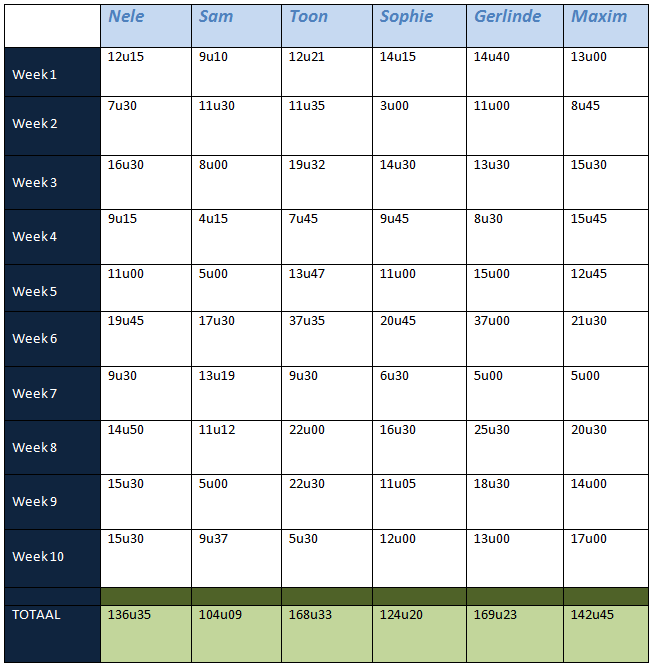
\includegraphics[width=0.8\textwidth]{werkschema}
    \caption{Het werkschema}
	\label{fig:werksch}
\end{center}
\end{figure}



 Geef voor elk van de groepsleden aan aan welke delen ze hebben meegewerkt en welke andere
taken ze op zich hebben genomen.
 Rapporteer in tabelvorm hoeveel uur elk groepslid elke week aan het project gewerkt heeft,
zowel tijdens als buiten de begeleide sessies. Geef ook totalen per groepslid voor het volledige
semester.
\section{Kritische analyse}
\label{kritischeAnalyse}
 Maak een analyse van de sterke en zwakke punten van het project. Welke punten zijn vatbaar


\begin{thebibliography}{9}

\bibitem{mindstorms}
\textit{Lego Mindstorms}:  Een uitbreiding op de LEGO bouwstenen waarmee kleine, aanpasbare en programmeerbare robots gebouwd kunnen worden. Een centrale besturingsmodule (`the brick') kan geprogrammeerd worden met verschillende programmeertalen. In eerdere versies werd een RCX gebruikt voor de brick, nu wordt met NXT gewerkt. De brick kan enkele motoren aandrijven. Bovendien kunnen er verschillende sensoren, o.a. een ultrasone sensor en een lichtsensor, aangesloten worden.  \mbox{[www.lego.com]} \mbox{[http://en.wikipedia.org/wiki/Lego\textendash Mindstorms]}

\bibitem{leJOS}
\textit{leJOS}: Een kleine Java Virtuele Machine die toelaat de NXT-brick te programmeren. leJOS voorziet verschillende klassen die o.a. de motoren aansturen en een bluetoothverbinding opzetten.  \mbox{[http://lejos.sourceforge.net/]}

\bibitem{A*}
\textit{A*}: Een optimaal zoekalgoritme. \textit{A*} kiest zijn volgende punt op basis van een kostenfunctie: de werkelijke kost om tot de beschouwde buur te geraken, plus de geschatte kost om van dat punt naar het doel te geraken. Met andere woorden, het algoritme combineert een heuristisch algoritme met een kostenalgoritme. Zie ook de cursus \textit{Artifici\"ele Intelligentie (H06U1A)} door Daniel De Schreye.

\bibitem{manhattan}
\textit{Manhattanafstand:} Deze heuristiek tekent vanuit het ene punt een horizontale lijn en vanuit het andere punt een verticale lijn. De gemeten afstand is die van het ene punt tot het snijpunt, plus die van het andere punt tot het snijpunt.\\
In de doolhof wordt geen rekening gehouden met muren.\\
De Manhattanafstand verwijst naar een gelijknamige stadsdeel in New~York~City~VSA). New~York werd in het jaar~1625 door de Nederlanders gesticht. De straten werden in dambordpatroon gelegd: `Avenues' van noord naar zuid en `Streets' van oost naar west.\\
\mbox{$[http://nl.wikipedia.org/wiki/Manhattan\_(New\_York)]$}\\ \mbox{$[http://nl.wikipedia.org/wiki/New\_York\_City]$}


\bibitem{Bag.java}
\textit{Bag}: Een manier om objecten op te slaan. Het is mogelijk te itereren over de verzameling, maar het is niet mogelijk objecten te verwijderen uit de verzameling. Meer documentatie: Section 1.3 of \textit{Algorithms, 4th Edition} door Robert Sedgewick en Kevin Wayne.\\
\mbox{[http://algs4.cs.princeton.edu/13stacks]} \mbox{[http://algs4.cs.princeton.edu/13stacks/Bag.java.html]}
\end{thebibliography}

\end{document}

